\section{Energia}

A solução de energia do projeto consiste no dimensionamento de baterias que atendam às especificações e requisitos do sistema, tanto dos dispositivos eletrônicos quanto do sistema de ignição, além disso será projetado um carregador de bateria para tornar contínuo o uso do equipamento.

Para dimensionar consumo do sistema, foi observado o gasto energético dos componentes eletrônicos levando em conta que o projeto precisa de uma autonomia de, no mínimo, duas horas de uso sem a possibilidade de ter como fonte de energia a rede elétrica.

\subsection{Consumo dos componentes}

Na tabela \ref{tab:consumo} é apresentado o consumo dos principais componentes elétricos e eletrônicos do sistema levantados até agora.

\begin{center}
\begin{table}[H]
\centering
\begin{tabular}{ |m{5cm}|m{3cm}|m{3cm}|m{3cm}| } 
\hline
\textbf{ Componentes }&\textbf{ Tensão} & \textbf{Corrente }& Potência \\ 
 \hline
 Tela & 12V & 1A & 12W \\
  \hline
Jetson Nano Developer Kit & 5V & 2A & 10W \\
  \hline
 Teclado e botões & 5V & 250 mA & 1,25W \\ 
  \hline
 Altímetro & 3V & 1 $\mu$ A & 3 $\mu$ W \\ 
 \hline
 GPS & 5V & 10mA & 500mW \\
 \hline
 Balança (célula de carga) & 10V & 100mA & 1W \\ 
 \hline
 Módulo base & 5V & 500mA & 2,5W \\ 
 \hline
 Módulo foguete & 5V & 500mA & 2,5W \\  
 \hline
 Módulo maleta & 5V & 500mA & 2,5W \\ 
 \hline
\end{tabular}
\caption{Consumo elétrico dos componentes.}
\label{tab:consumo}
\end{table}
\end{center}


\subsection{Alimentação}
Para a alimentação dos componentes, vão ser utilizadas tensões contínuas de 3 V, 5 V, 10 V e 12 V. A bateria a ser utilizada será de 12V, já que a maior tensão dentre todos os equipamentos é da tela de 12 V.

\subsubsection{ Cálculo para autonomia do sistema}
    
Para calcular a capacidade da bateria necessária para alimentar o sistema, são necessários os seguintes dados:
    \begin{itemize}
        \item Somatório de potência de todos os equipamentos.
        \item Tempo em horas de operação do sistema de maneira autônoma.
    \end{itemize}

Como especificado na tabela \ref{tab:consumo}, o somatório de potências do sistema é de 32,25 W. Será utilizado o valor de 35 W por segurança. O lançamento de um foguete tem duração média de 2 horas, o valor utilizado será de 3 horas, por segurança.

Sendo assim, o somatório da potência é multiplicado pelo tempo em horas.

\begin{center}
\begin{equation}\label{m}
	35 \times 3 = 105 Wh (Watts hora) 
\end{equation}
\end{center}

Essa será a energia necessária consumida para a autonomia especificada.

Pela Lei de Ohm temos: 
\begin{center}
\begin{equation}
\label{Lei de Ohm}
 I = \frac{P} {V}
\end{equation}
\end{center}

%$$ I = P/V $$

Onde, P se refere a potência, V a tensão e I a corrente.
\begin{center}
\begin{equation}
%\label{eq_vel_media}
 I = \frac{105} {12} = 8,75 Ah (Ampères hora)
\end{equation}
\end{center}


|%$$ I = 105/12 = 8,75 Ah (Ampères hora) $$

De acordo com o fabricante a capacidade da bateria deve ser mantida entre 50\% - 60\%, por segurança e de forma a prolongar a vida útil do equipamento \cite{datasheet_bateria}. Considerando então uma descarga máxima de 40\% a capacidade da bateria será:
\begin{center}
\begin{equation}
%\label{eq_vel_media}
\textbf{Capacidade em Ah } = \frac{8,75} {0,4} = 21,875 Ah
\end{equation}
\end{center}
%\textbf{Capacidade em Ah = 8,75/0,4 = 21,875 Ah}

Nos catálogos dos fabricantes pesquisados a capacidade mais próxima encontrada é de 30Ah.
Dessa forma será utilizada uma bateria com capacidade de \textbf {30 Ah}.

\subsection{Bateria}

Dentre os tipos mais comuns de baterias estão as de chumbo-ácido, de níquel-cádmio, de de níquel-hidreto metálico e de íons de lítio. Na Figura \ref{fig:tipos baterias} é apresentada uma comparação das características mais comuns dessas baterias \cite{artigo_bateria}.

\begin{figure}[!h]
	\centering
	\label{tipo de bateria}
		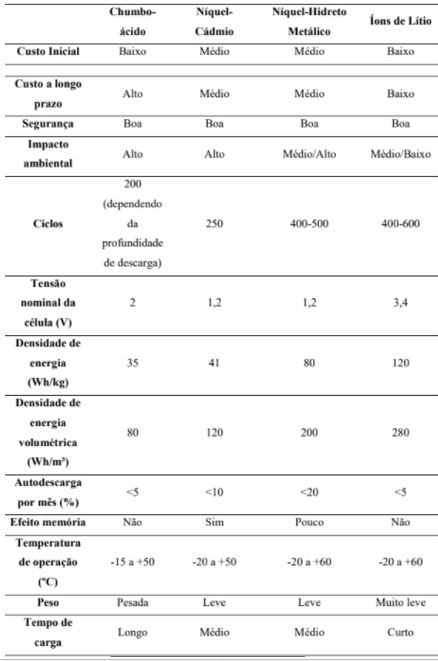
\includegraphics[keepaspectratio=true,scale=1]{figuras/Tabela_comparação_baterias.JPG}
	\caption{Características comuns de baterias.}
	{\footnotesize Fonte: \cite{artigo_bateria}}
	\label{fig:tipos baterias}
\end{figure}

Para o tipo de sistema em questão, algumas características são muito importantes para selecionar adequadamente a bateria a ser utilizada. A principal delas diz respeito ao peso e tamanho, como se trata de um sistema portátil se faz necessário selecionar uma bateria o mais leve e compacta possível. Além disso, o sistema será fundamentado no princípio de carregamento e descarregamento. Sendo assim, é importante selecionar uma bateria que permita diversos ciclos em sua vida útil e que não possua efeito memória (que diminui a capacidade de carga). As características que se referem a custo e impacto ambiental também são pontos relevantes para a escolha do tipo de bateria e para o projeto como um todo.

A partir da análise dos pontos mais importantes para o sistema dimensionado em comparação com as características encontradas na Figura \ref{fig:tipos baterias}, optou-se por utilizar uma bateria de Lítio. Os parâmetros da bateria já haviam sido calculados anteriormente, dessa forma, a bateria selecionada é uma bateria de Lítio de 12V e capacidade de 30Ah.

Durante as pesquisas para selecionar o fabricante, encontrou-se informações mais completas do fabricante \textit{Unipower}, da Bateria Lítio Ferro Fosfato - LiFePO4, modelo UPLFP12-30. As especificações estão descritas na Figura \ref{fig:caracteristica bateria} \cite{datasheet_bateria}.

\begin{figure}[!h]
	\centering
	\label{Características_bateria}
		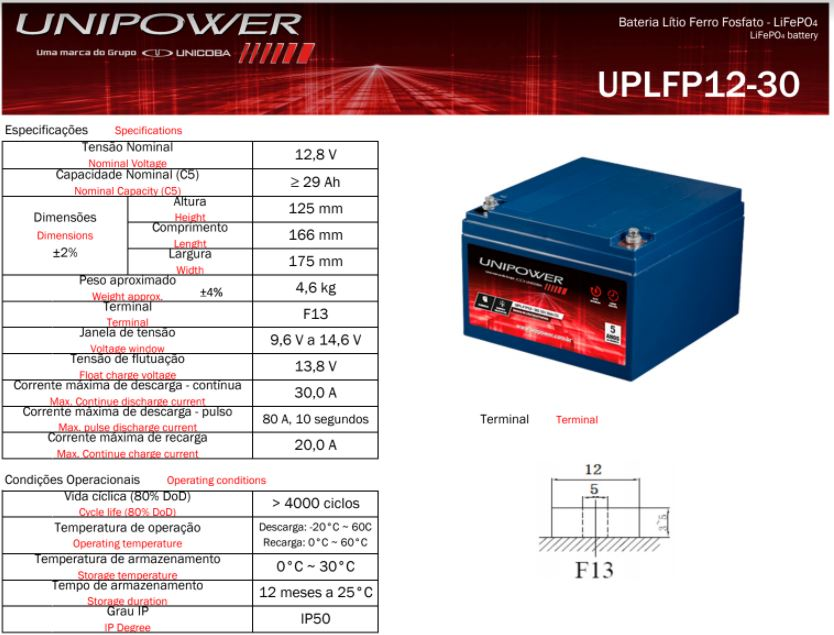
\includegraphics[keepaspectratio=true,scale=0.6]{figuras/Caracteristicas_bateria.JPG}
	\caption{Características técnicas da bateria escolhida. }
	{\footnotesize Fonte: \cite{datasheet_bateria}}
	\label{fig:caracteristica bateria}
\end{figure}


\subsection{Regulador de tensão}

Como a fonte de tensão é de 12V, serão utilizados módulos “\textit{step down}” para regular as tensões direcionadas para alguns componentes do sistema. No projeto, será utilizado o módulo regulador de tensão modelo LM2596 apresentado na figura \ref{fig:regulador tensao}, pois este possui uma ampla faixa de tensões de entrada e pode ser regulado para uma tensão específica de saída com uma boa eficiência \cite{datasheet_regulador}.

As faixas de tensão usadas serão de 3V, 5V e 10V de acordo com a necessidade de cada dispositivo eletrônico no sistema.

\begin{figure}[!h]
	\centering
	\label{regulador_tensão}
		\includegraphics[keepaspectratio=true,scale=1]{figuras/regulador_de_tensão.jpg}
	\caption{Regulador de tensão modelo LM2596.}
	\label{fig:regulador tensao}
\end{figure}

\subsection{Carregador de bateria}

A solução inicial para o sistema consistia em realizar o carregamento da bateria \textit{off grid}, ou seja, sem conexão com a rede elétrica, a partir do uso de placas fotovoltaicas. Porém, ao analisar as condições de operação do sistema, em especial o tempo de operação, que é previsto para no máximo 2 horas, concluiu-se que a solução mais adequada seria realizar o carregamento \textit{on grid}, conectado à rede elétrica, a partir de um carregador de bateria, a ser projetado.

Dessa forma, a bateria será levada com carga completa até o local de lançamento, todo o sistema poderá ser alimentado a partir dela, e, ao retornar para um local com conexão à rede elétrica a bateria poderá ser recarregada e o sistema estará pronto para o próximo uso.

O carregador a ser projetado deve seguir as especificações técnicas da bateria, a tensão de saída deve ser de 12V e a corrente máxima de saída 20A. Quanto aos parâmetros de alimentação da rede, como o lançamento não se restringe a região de Brasília e pode acontecer em diferentes locais do país, o carregador deve suportar uma tensão de entrada entre 100V e 240V.


